\documentclass[a4paper]{article}
\usepackage[spanish]{babel}
\usepackage[utf8]{inputenc}
\usepackage{charter}   % tipografia
\usepackage{graphicx}
%\usepackage{makeidx}
\usepackage{paralist} %itemize inline
\usepackage{pdfpages}


%\usepackage{float}
%\usepackage{amsmath, amsthm, amssymb}
%\usepackage{amsfonts}
%\usepackage{sectsty}
%\usepackage{charter}
%\usepackage{wrapfig}
%\usepackage{listings}
%\lstset{language=C}


\usepackage{color} % para snipets de codigo coloreados
\usepackage{fancybox}  % para el sbox de los snipets de codigo

\definecolor{litegrey}{gray}{0.94}

% \newenvironment{sidebar}{%
% 	\begin{Sbox}\begin{minipage}{.85\textwidth}}%
% 	{\end{minipage}\end{Sbox}%
% 		\begin{center}\setlength{\fboxsep}{6pt}%
% 		\shadowbox{\TheSbox}\end{center}}
% \newenvironment{warning}{%
% 	\begin{Sbox}\begin{minipage}{.85\textwidth}\sffamily\lite\small\RaggedRight}%
% 	{\end{minipage}\end{Sbox}%
% 		\begin{center}\setlength{\fboxsep}{6pt}%
% 		\colorbox{litegrey}{\TheSbox}\end{center}}

\newenvironment{codesnippet}{%
	\begin{Sbox}\begin{minipage}{\textwidth}\sffamily\small}%
	{\end{minipage}\end{Sbox}%
		\begin{center}%
		\vspace{-0.4cm}\colorbox{litegrey}{\TheSbox}\end{center}\vspace{0.3cm}}



\usepackage{fancyhdr}
\pagestyle{fancy}

%\renewcommand{\chaptermark}[1]{\markboth{#1}{}}
\renewcommand{\sectionmark}[1]{\markright{\thesection\ - #1}}

\fancyhf{}

\fancyhead[LO]{Sección \rightmark} % \thesection\ 
\fancyfoot[LO]{\small{Aldasoro Agustina, Bouz\'on Mar\'ia Bel\'en, Cairo Gustavo Juan}}
\fancyfoot[RO]{\thepage}
\renewcommand{\headrulewidth}{0.5pt}
\renewcommand{\footrulewidth}{0.5pt}
\setlength{\hoffset}{-0.8in}
\setlength{\textwidth}{16cm}
%\setlength{\hoffset}{-1.1cm}
%\setlength{\textwidth}{16cm}
\setlength{\headsep}{0.5cm}
\setlength{\textheight}{25cm}
\setlength{\voffset}{-0.7in}
\setlength{\headwidth}{\textwidth}
\setlength{\headheight}{13.1pt}

\renewcommand{\baselinestretch}{1.1}  % line spacing


% \setcounter{secnumdepth}{2}
\usepackage{underscore}
\usepackage{caratula}
\usepackage{url}




\begin{document}


\thispagestyle{empty}
\materia{M\'etodos Num\'ericos}
\submateria{Segundo Cuatrimestre de 2014}
\titulo{Trabajo Práctico III}
\subtitulo{Develando la mentira de los megap\'ixeles}
\integrante{Aldasoro Agustina}{86/13}{agusaldasoro@gmail.com}
\integrante{Bouz\'on Mar\'ia Bel\'en}{128/13}{belenbouzon@hotmail.com}
\integrante{Cairo Gustavo Juan}{89/13}{gjcairo@gmail.com}

\maketitle
\newpage

\thispagestyle{empty}
\vfill
\begin{abstract}
En el presente trabajo se pretende analizar y comparar distintas alternativas que pretenden dar respuesta al problema de demosaicing. Para ello, las mismas serán implementadas y sometidas a experimentación sobre fotografías crudas sintéticas específicamente seleccionadas para poner de manifiesto las ventajas e inconvenientes del empleo de cada método. \\
\end{abstract}

\textbf{Palabras clave:} \\
$\bullet$ Filtro Bayer \\
$\bullet$ Demosaicing \\
$\bullet$ Interpolaci\'on \\
$\bullet$ Artifacts \\



\thispagestyle{empty}
\vspace{3cm}
\tableofcontents
\newpage


%\normalsize
\newpage

\section{Introducci\'on Te\'orica}

Promediando la década de 1990 comenzaron a introducirse al mercado las cámaras digitales de uso hogareño, empezando a sustituir desde entonces a las ampliamente difundidas cámaras de film. 
Mientras que estas últimas capturaban la imagen de forma mecánica y sin intercesión de un procesamiento digital (\textcolor{red}{¿? Asegurarse cómo es y explayarse. Estuve buscando y no entendi o no encontre nada. me parece que asi esta bien}), las cámaras electrónicas emplearon una nueva tecnología. Esta tecnolog\'ia distingue entre en el momento de obtención de un conjunto de datos cerca del objetivo – donde se obtiene una imagen que llamaremos “\textit{cruda}” – y una etapa de procesamiento automático conjunto a la reconstrucción de la imagen final. \\

En el presente trabajo nos interesará analizar un fragmento de dicha etapa conocido como \emph{demosaicing}. Para entender de qué consta, es menester comprender previamente la forma en que se capturan las imágenes al utilizar cámaras digitales.

Este tipo de cámaras poseen un sensor CCD compuesto de una matriz de elementos fotosensibles, cada uno de los cuales es capaz de captar la intensidad de la luz que llega a ese punto a través de la lente. 

La tarea de capturar todos los colores reflejados por el objetivo que se quiere fotografiar no está encomendada a ninguna posición en particular, sino que cada una de ellas tiene asignada – de acuerdo a algún patrón definido  – la captura de la información perteneciente a un solo color. Cada p\'ixel de la imagen va a estar dividido en tres canales ya que la vamos a almacenar mediante RGB (Red, Green, Blue).

Ahora bien, esto genera una imagen que se aproxima a la realidad sólo en parte ya que para cada p\'ixel de la imagen tenemos la informaci\'on de s\'olo uno de sus tres canales. A causa de esto es que la misma debe ser reconstruida algorítmicamente, interpolando los valores de los colores que no fueron almacenados explícitamente para cada pixel.

%El patr\'on que determina qué color será capturado por cada fotosensor es denominado \textbf{Color Filter Array} y var\'ia de acuerdo al fabricante de c\'amaras %%%%digitales. En nuestro trabajo nos centraremos en el \textbf{Filtro Bayer}, ya que es un filtro com\'unmente usado debido a que la cantidad de informaci\'on que brinda% sobre el canal verde - al cual el ojo humano es m\ás sensible, debido a que se encuentra en el centro de su espectro visual - duplica a cada uno de los otros dos. 

\textcolor{blue}{*insertar imágenes por aquí y por allá*}

En este punto adquieren relevancia las diferentes propuestas de reconstrucción de la imagen original. Esto conlleva la ejecución de diversos procedimientos, entre los que se encuentran el demosaicing, el análisis del balance de blancos, la curva tonal, la saturación y el contraste y la compresión final de la imagen. Como nuestra propuesta se aboca al primer paso mencionado, exploraremos en el presente trabajo sólo un subconjunto de una serie de variaciones no finita que admiten métodos de debayering como ser la interpolación por asignación de valores próximos, la interpolación bilineal y interpolación direccional.\\


\newpage
\section{Desarrollo}

Dada una \textit{imagen cruda}, los valores que contiene en sus píxeles para cada canal los asumimos reales y ciertos. Por lo tanto, resta averiguar para cada uno de ellos los valores de los dos canales para los cuales dicha información se encuentra ausente.

\subsection{Vecino m\'as cercano}
La implementación más sencilla para la estimación de los canales desconocidos de cada pixel consiste en otorgar a cada canal ``vacío'' el valor real m\'as pr\'oximo que corresponda a dicho color. Este m\'etodo es algor\'itmicamente asequible, pero no tiene en cuenta dos factores: \\
\\
$\triangleright$ Por un lado, al otorgar el valor de un sólo pixel cercano, surge la necesidad de definir arbitrariamente cuál se debe escoger como valor referencial en casos en que un conjunto de pixeles son equidistantes al analizado y no existe un criterio claro acerca de cuál de ellos debe ser considerado el ``más próximo''. Que esta decisión impacte en el resultado de forma inocua o parcial o totalmente nociva dependerá en cierta medida de la fotografía que se esté analizando.\\
El ejemplo más trivial se encuentra en una imagen monocromática: al ser los valores reales idénticos para todos los pixeles, tomar las magnitudes de cualquier otra posición para cada canal correspondiente no afectará el resultado final. Sin embargo, si consideráramos una imagen formada por columnas alternadas de un pixel de ancho rojas (\#0000FF) y blancas (\#FFFFFF), entonces si para definir los canales verde y azul de un pixel rojo se tomara como posiciones más cercanas aquel que se encuentra debajo suyo y el que está a la derecha del mismo (respectivamente), el resultado sería un pixel fucsia (\#FF00FF). En cambio, si los pixeles elegidos fueran su inmediato derecho y en el que se encuentra a su diagonal inferior derecha, la posición analizada debería manifestar el color blanco (\#000000).\\
Si bien se trata de un ejemplo de alcance limitado, resulta suficiente para ilustrar los potenciales problemas de la aplicación de este algoritmo.
\\
$\triangleright$ Por otra parte - y en cierta forma vinculado al ejemplo anterior - este método no especifica ninguna distinción respecto de la forma de proceder en casos de borde o de superficies parejas. \\

\subsection{Interpolaci\'on Bilineal}

%La interpolación bilineal es una composición de interpolaciones lineales en dos direcciones diferentes. Este método desmerece el caracter arbitrario de asignación de un canal a partir del valor más pr´ximo para el mismo y propone que el resultado final sea calculado teniendo en cuenta y promediando todos los valores cercanos sin priorizar ninguno de ellos. \\
Como la estructura del filtro Bayer sólo asegura para los pixels nativamente azules o rojos tener todas sus posiciones vecinas netamente verdes , aquel es el único caso en que el cálculo de un canal se reduce a computar el promedio de los valores superior, inferior, derecho e izquierdo al espacio que se quiere interpolar.\\
Sin embargo, si se quisiera obtener el valor de azul o rojo que correspondería asignar a un pixel nativamente verde, el entramado de Bayer obligaría a estimarlo a partir de los valores de la columna o de la fila, respectivamente, puesto que la intersección entre las columnas que capturan el color rojo y el verde y las que toman este último junto al azul es vacía.\\
Por otro lado, los valores del canal azul para un pixel rojo (y los del canal rojo para un pixel azul) se calcularían tomando en cuenta las posiciones diagonales a la analizada. Esto requeriría tomar dos pixels cercanos cuyo canal real sea el verde y cuyas filas/columnas resulten paralelas entre sí, calcular sus valores de azul/rojo promediando los de las casillas nativas azules/rojas más próximas y posteriormente realizar un nuevo promedio entre los valores resultantes.\\
Tomando como referencia la ilustración \ref{bilineal} se puede ver que el cálculo recien descripto equivale a definir el promedio entre los valores diagonales más cercanos, puesto que ((a+b)/2 + (c+d)/2)/2 = (a+b+c+d)/4.

\begin{figure}[h!]
	\caption{}
	\begin{center}
	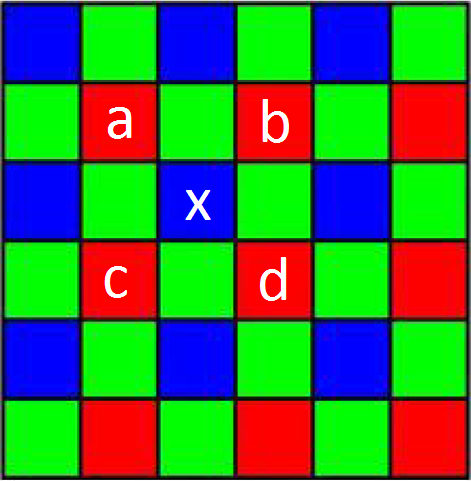
\includegraphics[scale=0.36]{imagenes/bilineal}
	\label{bilineal}
  \end{center}
\end{figure}


\subsection{Interpolaciones Direccionales}
Se trata de una gran cantidad de métodos que buscan comenzar a resolver el problema de demosaicing realizando inicialmente una interpolación en una dirección y combinando con algún criterio determinado el resultado estimado con el obtenido de una aproximación realizada en otra dirección.\\

La implementación de este tipo de métodos exige tomar al menos dos decisiones de peso que distinguirán a unos de otros:\\

\begin{itemize}
    \item De qué forma se realizarán las interpolaciones (en qué direcciones y mediante qué mecanismo de interpolación)
    \item Con qué criterio y consideraciones combinar la información proporcionada por las direcciones escogidas.
\end{itemize}

Para escoger alguna opción apropiada corresponde analizar las características del Color Filter Array con el que se va a trabajar, puesto que no todas las direcciones van a aportar en la totalidad de los casos la misma información. \\
En cuanto a la combinación de los resultados de las distintas interpolaciones, es conveniente tener presente que el promedio de los mismos no es siempre una buena opción. Por ejemplo, supongamos que se analiza una imagen que presenta en un sector la siguiente característica:

\begin{figure}[h!]
	\caption{}
	\begin{center}
	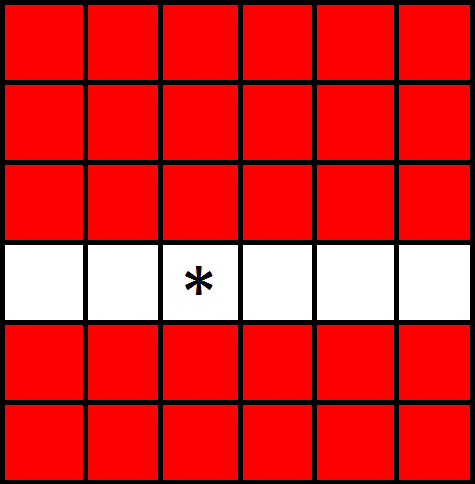
\includegraphics[scale=0.26]{imagenes/direccional}
	\label{direccional}
  \end{center}
\end{figure}

Si se interpolara utilizando la dirección vertical el valor de la posición denotada con una estrella, todo indicaría que el resultado debería generar el color rojo. Al hacerlo horizontalmente se llegaría a la conclusión de que la posición en cuestión debería ser blanca. Promediando \#FF0000 con \#FFFFFF resultaría el valor \#FF8080, que expresa un color rosado. \\
Ciertamente esto no es lo esperado y existen mecanismos que permiten corregir este error. Uno de ellos consiste en calcular el gradiente del color para utilizarlo al combinar los resultados, de modo tal que si el mismo fuera de gran magnitud (es decir, la variación del color es considerable) entonces el peso que debe tener el valor calculado en el resultado final debería ser menor a aquel que fue calculado en una dirección cuyo gradiente fuera menor (es decir, que se tratara de una superficie más cromáticamente homogénea).

\textcolor{red}{No sé qué más poner acá =/ re cortina.-}


\subsection{Algoritmo de Malvar, He y Cutler}




\newpage
\section{Resultados y discusi\'on}
\subsection{MHC}
Le da muchísima más definición/claridad a las fotos, y los bordes oscuros quedan prácticamente perfectos (comparando con bilineal, por ejemplo, aparecen colores fuertes alrededor de los bordes negros). Sigue pasando eso con los bordes blancos/mas claros, pero las zonas donde hay un salto grande entre claro y oscuro, mejora mucho.

\newpage
\section{Conclusiones y trabajo futuro}





\section{Ap\'endices}
\subsection{Ap\'endice A: Enunciado} 
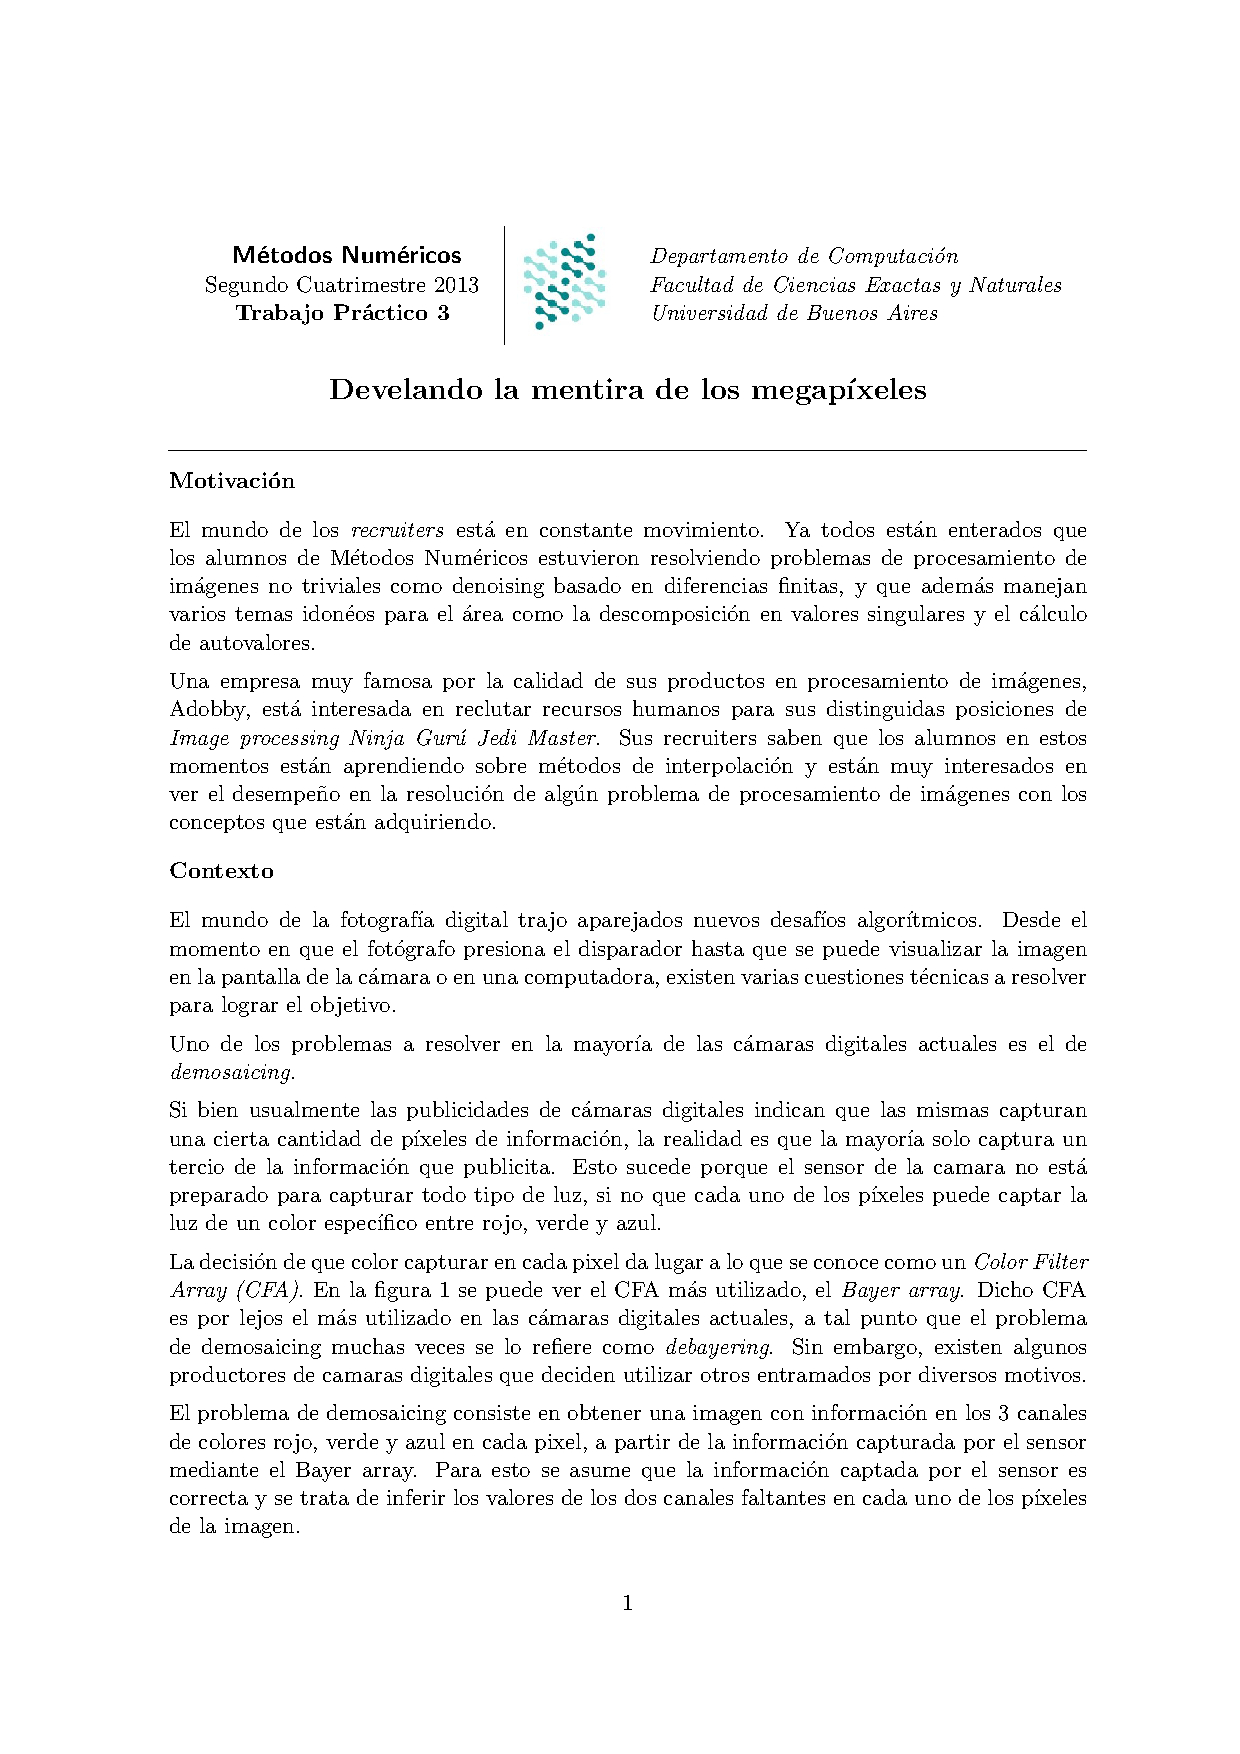
\includepdf[pages={-}]{Enunciado.pdf}

\subsection{Ap\'endice B:}
\newpage
\section{Referencias}
 
\textbf{[1]} Ron Kimmel. Demosaicing: image reconstruction from color ccd samples. \textit{IMAGE PROCESSING, IEEE TRANSACTIONS ON}, 1999. \\
\\

\textbf{[2]} Henrique S. Malvar, Li wei He, and Ross Cutler. High-quality linear interpolation for
demosaicing of bayer-patterned color images. In \textit{Proceedings of the IEEE International
Conference on Speech, Acoustics, and Signal Processing}, 2004.

\end{document}

%%%%%%%%%%%%%%%%%%%%%%%%%%%%%%%%%%%%%%%%%%%%%%%%%%%%%%%%%%%%%%%%%%%%%%%%%
\begin{figure}
  \begin{center}
	
\includegraphics[scale=0.66]{imagenes/logouba.jpg}
	\caption{Descripcion de la figura}
	\label{nombreparareferenciar}
  \end{center}
\end{figure}


\paragraph{\textbf{Titulo del parrafo} } Bla bla bla bla.
Esto se muestra en la figura~\ref{nombreparareferenciar}.



\begin{codesnippet}
\begin{verbatim}

struct Pepe {

    ...

};

\end{verbatim}
\end{codesnippet}
